
\chapter{Application of Algorithms}
In this chapter the main algorithms that were covered in chapter \ref{chp:vision} are going to 
be examined in a more practical fashion. The algorithms will 
be prototyped against the navigation scenario in a net.

As mentioned in section \vref{sec:high_def_video_analysis} all implementations done uses the open source \gls{ocv} library. This is done 
through the \gls{python} bindings made available by the project for prototyping, and through the \gls{cpp} API to see how 
the runtime of the algorithms compare. By design, \gls{python} will be slower than the \gls{cpp} versions as \gls{python} is a 
interpreted and \gls{jit} based run time. This means that the \gls{python} runtime needs to perform \gls{marshalling} which 
gives a speed impact.

\section{Optical flow algorithms}

\subsection{Flow fields}
Lucas-Kanade is the main algorithm that tries to identify optical flow by modelling the difference between two frames as a flow field. This algorithm 
is described in section \vref{sec:lukas-kanade}. 

The version of Lucas-Kanade that were implemented is based on the pyramid version of the algorithm. This makes the 
algorithm less computational expensive. The pyramid is built up based on the \verb|cv::goodFeaturesToTrack| function in the OpenCV library. 
This function uses a Canny edge detector to detect features in a frame. This makes use of the fact that edge intersections 
normally does not deform between two frames. Features that are traceable will by that argument be in the 
concave section of two or more intersecting Canny lines.

The initialization of the feature points yields the image in figure \vref{fig:lk_1}. The red circles shows 
where the Canny detector has found strong enough line intersections.

\begin{figure}[htbp]
	\centering
	\includegraphics[width=\textwidth]{lk_pyramid_1}
	\caption{Initialization point of Lucas-Kanade. Red dots show the tracking result from the Canny Edge Detector.}
	\label{fig:lk_1}
\end{figure}

The problem with finding good enough features becomes evident after some time. Figure \vref{fig:lk_2} shows the 
tracking result after \SI{1}{\second}. Since the features needs to be constant to be tracked, no new features are found as masks in the net moves 
off the screen. This is mainly rooted in the normal application of algorithms such as this. Normally, the algorithm would be used to track either a single object or 
some discrete number of objects in a stream of frames. 

Applying the Lucas-Kanade algorithm however to the net scenario yields bad results. One reason is that the track points starts to slip on the features 
that were chosen to be tracked. The reason for this is the relative uniformity of the environment, which is not something that the Lucas-Kanade algorithm 
were designed to track. This is rooted in the velocity smoothness constraint mentioned in section \ref{sec:lukas-kanade} 

\begin{figure}
	\centering
	\includegraphics[width=\textwidth]{lk_pyramid_2}
	\caption{1 second of tracking using the Lucas-Kanade algorithm with the initialization from \ref{fig:lk_1}.}
	\label{fig:lk_2}
\end{figure}

\subsection{Energy fields}

\subsubsection{Horn-Schunck}
The main algorithm that uses energy fields to model the flow between two frames is the Horn-Schunck algorithm described in section \vref{sec:horn-schunck}. This 
algorithm has been more or less replaced by the \citet{farnebackSCIA03} algorithm, as described in section \vref{sec:farneback}. 

On this background, the Horn-Schunck 
algorithm were not implemented or tested. 
This is mainly because of the statistical data presented by \citet{farnebackSCIA03} showing that the 
Farnebäck algorithm never gives a worse result than the Horn-Schunck algorithm, while proving to be 
less computational expensive.

\clearpage

\subsubsection{Farnebäck}
Farnebäck became the algorithm with a base in the theory of energy fields that were implemented. This 
is quite a new algorithm in the field of optical flow, but it has proven itself to be 
quite a robust and attractive algorithm. The implementation is based on \citet{farnebackSCIA03} by 
using the \gls{ocv} library.

The image in figure \ref{fig:farneback_1} shows the field calculated 
by the algorithm during linear translation in a realistic scenario. This means 
that even though the majority of movement found goes in the 
downward direction. A close-up view can be seen in figure \ref{fig:farneback_2}.

\begin{figure}[htbp]
	\centering
	\includegraphics[width=\textwidth]{farneback_1}
	\caption{Using \citet{farnebackSCIA03} to track movement when net is lowered. Each point is the sum of movement in the 
		rectangle which the point is in the centre of that spans to a equidistant grid over the whole image.}
	\label{fig:farneback_1}
\end{figure}

\begin{figure}[htbp]
	\centering
	\includegraphics[height=\textwidth, angle=90]{farneback_2}
	\caption{Closer look at the output from \citet{farnebackSCIA03} on a subset of masks. Almost uniform flow 
		is detected in the points where the net movement happens. Up direction is to the left in the image.}
	\label{fig:farneback_2}
\end{figure}

Since this algorithm estimates the field in a grid, it can be 
sensitive to weak references and smoothing. A example of real life conditions 
that may lead to a loss of the field in areas with low contrast is shown in 
figure \ref{fig:farneback_3}.

\begin{figure}[htbp]
	\centering
	\includegraphics[width=\textwidth]{farneback_3}
	\caption{Overview of tracking. Note good tracking in points that contains the vertical parts of the masks and the loss of tracking in 
		the lover left corner.}
	\label{fig:farneback_3}
\end{figure}

Based on how the algorithm calculates the flow, it is also obvious that the Farnebäck algorithm 
is susceptible to other foreground objects that will distort the measurement of the flow for the net. 
This is based in the local grid that this algorithm uses, and it therefore does 
not use some global measurement to detect the mean flow. These features can be seen in figure \ref{fig:farneback_dist_1} and 
\ref{fig:farneback_dist_2}.

\begin{figure}[htbp]
	\centering
	\includegraphics[height=\textwidth, angle=90]{farneback_distortion_1}
	\caption{Showing \citet{farnebackSCIA03} tracking other unwanted objects in the stream. Here some small air bubble are being tracked. 
		Upwards direction is to the left in the image.}
	\label{fig:farneback_dist_1}
\end{figure}

\begin{figure}[htbp]
	\centering
	\includegraphics[width=\textwidth]{farneback_distortion_2}
	\caption{Showing \citet{farnebackSCIA03} tracking the bottom line of the rig. Multiple big distortions.}
	\label{fig:farneback_dist_2}
\end{figure}

The hard distortions seen if figure \ref{fig:farneback_dist_1} and 
\ref{fig:farneback_dist_2} stems from the intended use 
of the algorithm. It is optimized to find either global flow when 
the image only contains background, or to track objects in the foreground. 

The Farnebäck algorithm were tested on a sample video. The movement detected by
the algorithm has been plotted in figure \vref{fig:farneback_move}. Note that 
the dimensions for the movement are related by 
some scaling factor to the real movement in the image stream.

\begin{figure}[htbp]
    \centering
    \subfloat[Result of the Farnebäck algorithm detected movement on a sample video.]
    	{\label{fig:farneback_move_1}{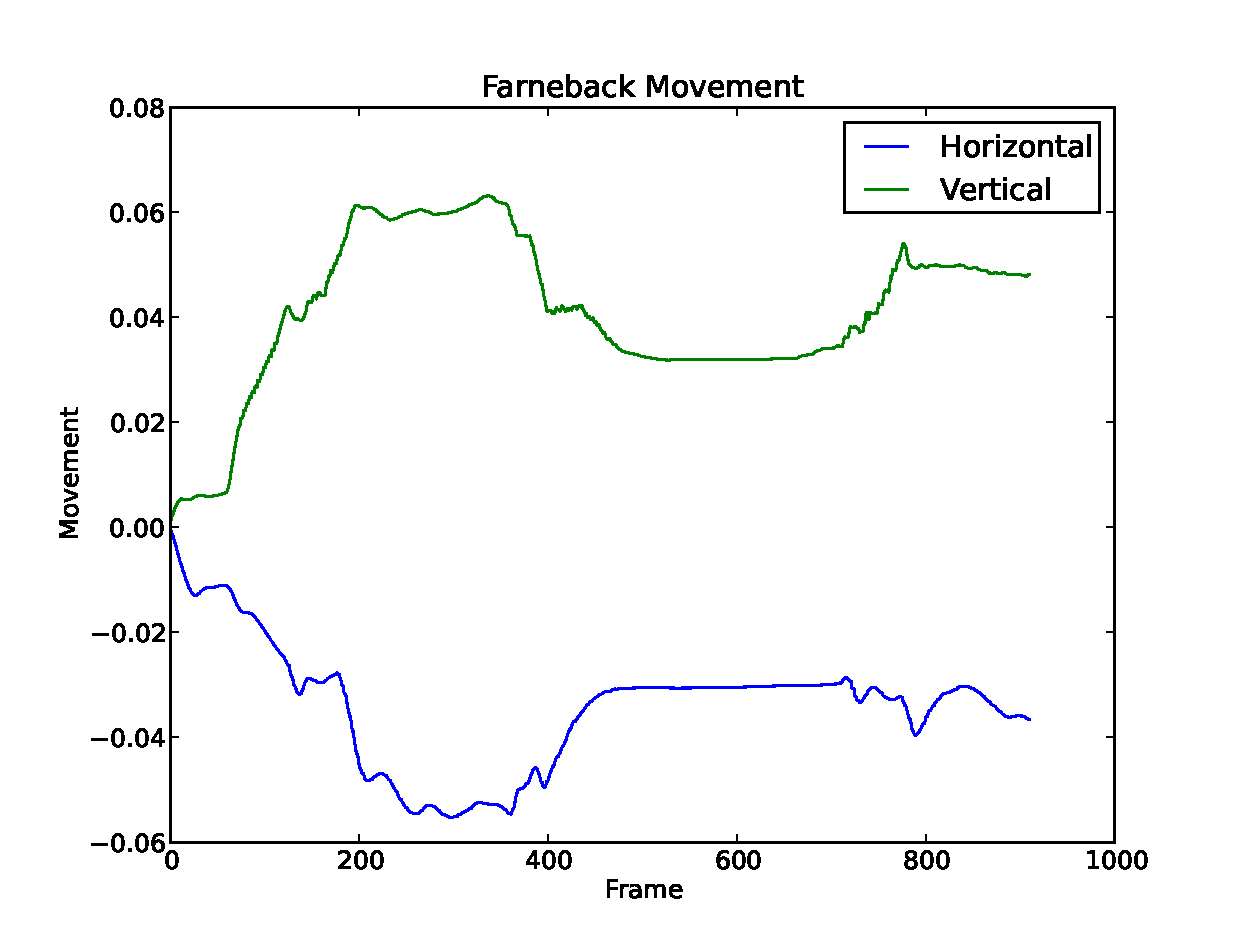
\includegraphics[width=0.8\textwidth]{farneback_move_1}}}
    \\
	\subfloat[Result of the Farnebäck algorithm detected movement on a sample video, horizontal position plotted against vertical position.]
		{\label{fig:farneback_move_2}{\includegraphics[width=0.8\textwidth]{farneback_move_2}}}
	\caption{Using the Farnebäck algorithm on a sample video. 
		Shown as position vs frame (\ref{fig:phase_run_1}) and x-position vs y-position (\ref{fig:phase_run_2}).}
	\label{fig:farneback_move}
\end{figure}

\clearpage

\subsection{Line tracing}
The use of Hough Transforms was tested by \citet{carlsen10} to detect the net and masks in the net. His trials were initially done in a 
static scenario with the net held in place by a metal frame. He showed that it was possible to find the lines describing the mask 
structure using the normal Hough Transform by setting strict parameters on the minimum distance between detected lines under those conditions.
It proved however to be much worse to get stable readings during his field test, and 

The image in figure \vref{fig:hl_1} shows the results of the normal Hough Transform on the net suspended in free water. Due to the 
movement of the net, and the folding seen in figure \ref{fig:hl_1} the transform fails to find a consistent number of lines. When  
the net starts moving up as shown in figure \ref{fig:hl_2} it seems as most of the lines that were found in figure \ref{fig:hl_1} 
is being tracked correctly. However, as the Hough Transform generates a new set of lines for each image this is not an assumption 
that generally holds. 

\begin{figure}[htbp]
	\centering
	\includegraphics[width=\textwidth]{houghlines_1}
	\caption{Initial result of the Hough Line Transform on a net at rest}
	\label{fig:hl_1}
\end{figure}

\begin{figure}[htbp]
	\centering
	\includegraphics[width=\textwidth]{houghlines_2}
	\caption{Result of the Hough Line Transform when the net is moving}
	\label{fig:hl_2}
\end{figure}

According to section \vref{sec:hough.transform.prob} the Probabilistic Hough transform would be a better choice in the
environment shown in figure \ref{fig:hl_1}. This comes from the design of the algorithm to not 
assume that lines are straight for the duration of the lines. Using the probabilistic properties from section \ref{sec:hough.transform.prob} 
the image in figure \vref{fig:hl_p_1} were obtained. This is from the same sequence as figure \ref{fig:hl_1}. The image in figure \ref{fig:hl_p_2}
is from the same sequence as figure \ref{fig:hl_2}, and shows how the probabilistic transform detects lines during movement.

\begin{figure}[htbp]
	\centering
	\includegraphics[width=\textwidth]{houghlines_probabilistic_1}
	\caption{Initial result of the Probabilistic Hough Line Transform on a net at rest}
	\label{fig:hl_p_1}
\end{figure}

\begin{figure}[htbp]
	\centering
	\includegraphics[width=\textwidth]{houghlines_probabilistic_2}
	\caption{Result of the Probabilistic Hough Line Transform when the net is moving}
	\label{fig:hl_p_2}
\end{figure}

\clearpage

\subsection{Phase correlation}
The Phase Correlation algorithm that were described in section \vref{sec:phase.correlation} were also tested. This 
is one of the older methods of finding flow, and it is mainly designed to find the linear translation between two frames.
The use of a phase plane makes the algorithm extremely resilient to noise in the image. This is in sharp contradiction 
to other algorithms that work in the spatial domain.

\begin{figure}[htbp]
    \centering
    \subfloat[Result of Phase Correlation detected movement on a sample video.]
    	{\label{fig:phase_run_1}{\includegraphics[width=0.8\textwidth]{phase_run_1}}}
    \\
	\subfloat[Result of Phase Correlation detected movement on a sample video, horizontal position plotted against vertical position.]
		{\label{fig:phase_run_2}{\includegraphics[width=0.8\textwidth]{phase_run_2}}}
	\caption{Using Phase Correlation on a sample video. 
		Shown as position vs frame (\ref{fig:phase_run_1}) and x-position vs y-position (\ref{fig:phase_run_2}).}
	\label{fig:phase_run}
\end{figure}

The output from the phase correlation algorithm is the primary detected movement between two frames, and some 
statistical data about the detected movement. This means that it is easily 
plotted as shown in figure \ref{fig:phase_run}. 

The figures in figure \ref{fig:phase_run} shows the 
same video sequence plotted in two different ways. Figure \ref{fig:phase_run_1} shows the two 
different dimensions of the video and how it is detected to move during the full duration of the stream. This gives a temporal 
view of how the movement progresses. Figure \ref{fig:phase_run_2} shows a polar plot of the same, where the horizontal and vertical 
components  This plot loses the temporal component, but it shows a trace of the 
movement of the net. 
